Modelling refers to the process of creating a simplified representation or
approximation of a real-world system, process, or phenomenon in order to improve
understanding and facilitate analysis.~It is commonly used in the fields of
physics and mathematics, where mathematical equations are used to depict reality
and capture the important factors of a particular system in a manageable and
understandable format~\cite{witelski2015methods}.

In the field of optimization, there is an extensive body of literature on the
development of glass-box~\acrshort{ilp} models for a wide range of
problems~\cite{papadimitriou1998combinatorial,nocedal2006numerical,williamson2011design}.
One of the key advantages of this approach is that it allows for the application
of standard solvers that can be used to find solutions to diverse problems. This
can be attributed to the fact that the model encapsulates all the information
required by a generic solver,~\eg{},\textit{Gurobi},~\textit{CPLEX},
or~\textit{GLPK}, to address any problem in a principled manner.

As an example of this~\acrshort{glass-box-optimization} modelling approach
consider the~\acrshort{knapsack-problem} for which an~\acrshort{ilp}
model~\cite{yu2010combinatorial} is represented by the
formulation~\ref{eq:knapsack-ilp}.~Herein, the parameter $n$ signifies the count
of items, while $W$ designates the knapsack's maximum capacity.  Additionally,
the variables $w_{i}$ and $p_{i}$ correspond to the weight and profit,
respectively, associated with each individual item $i$. Furthermore, the binary
variable $x_{i}$ is employed to denote whether a particular item is included
(assigned a value of 1) or excluded (assigned a value of 0) from the knapsack,
for a given solution.

\begin{equation}
      \label{eq:knapsack-ilp}
      \begin{aligned}
            \max f(x) = & \sum_{i=1}^{n} p_i \cdot x_i                           \\
            \text{s.t } & \sum_{i=1}^{n} w_i \cdot x_i \leq W                    \\
                        & x_i \in \{0, 1\} \quad \text{for } i = 1, 2, \ldots, n
      \end{aligned}
\end{equation}

It's crucial to recognize that this formulation highlights several significant
aspects of the problem.~These include the decision space, which defines the
range of values each variable can take; the objective function, which expresses
the optimization goal; the construction rules (constraints) that guide the
creation of a valid solution; and the problem instance parameters necessary for
defining and solving the problem instance effectively.

When approaching problems from a~\acrshort{black-box-optimization} perspective,
particularly through \acrshort{meta-heuristic} solvers, the notion of developing
a reusable model has yet to be established, as far as our knowledge extends.
However, for such a model to come into existence, it would need to address, at
the very least, the same details as the
aforementioned~\acrshort{knapsack-problem} model.~Furthermore, considering the
strategies employed by~\acrshort{meta-heuristic} solvers to explore
solutions~(\Cref{sec:meta-heuristics}), certain recurring aspects emerge as
essential questions that a model must address:

\begin{description}
      \item[\textbf{Problem Instance.}] What information is required to characterize a particular problem (instance)?
      \item[\textbf{Solution.}] How do we characterize an empty, partial or complete solution for the problem, and its feasibility?
      \item[\textbf{Objective Function \& Bounds.}] Can we evaluate a partial or complete solution, and how? How do we calculate the bounds for a (partial) solution?
      \item[\textbf{Combinatorial Strutcture (\acrshort{constructive-search}).}] How do we construct solutions? What is the ground set, components and how are they added/removed to/from the solution.
      \item[\textbf{Neighborhood Strutucture (\acrshort{local-search}).}] How do we characterize neighborhood of a solution and the possible local moves?
\end{description}

Incorporating a standardized approach to address these fundamental questions can
pave the way for a systematic problem-solving methodology. This enables the
integration of meta-heuristics as powerful solvers, akin to traditional solvers
in mathematical programming. This approach diverges from existing meta-heuristic
frameworks~\cite{cahon2004paradiseoa,digaspero2003easylocal,durillo2011jmetal},
where custom meta-heuristic solvers are tailored for each specific problem.
Instead, it establishes a problem-independent abstraction layer (model) that
equips solvers with essential information across diverse meta-heuristics, while
abstracting the intricacies of inherent to each specific problem.

\begin{figure}[h]
      \centering
      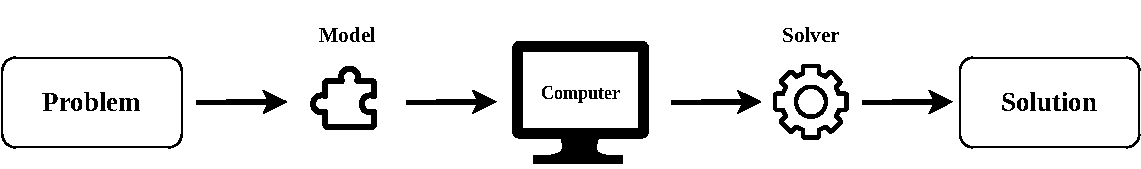
\includegraphics[width=\textwidth,keepaspectratio]{../assets/modelling/modelling.pdf}
      \caption{Principled Modelling Framework}
      \label{fig:pmf}
\end{figure}

The overall concept for a principled meta-heuristics modeling framework is to
create a standardized model that is applicable to any problem domain. This model
comprises a set of functions that encapsulate the essential aspects of the
problem. This model is then provided to a computer system, which employs a range
of meta-heuristics. These meta-heuristics utilize the set of functions within
the model to effectively generate solutions, as illustrated in~\Cref{fig:pmf}.

Crucially, the set of functions represents the core of the standardized model.
An essential consideration is to refine this set of functions to capture the
fundamental characteristics that are universally present in all problems. This
avoids the need for distinct functions for each problem, which would defeat the
purpose of creating a standardized approach.

Notably, this framework for tackling problems in the context of meta-heuristics,
which we refer to as the principled modelling approach, has been seldomly
researched and constitutes an ongoing research effort. In fact, we identify two
noteworthy studies in the literature and three attempts in practically
developing an~\acrfull{api} for this modelling
framework~\cite{vieira2009uma,outeiro2021application,fonseca2021nasf4nio}.

\subsection{Software}

The first attempt at developing a modeling framework for experimental testing of
meta-heuristics can be traced back to the pioneering thesis work
of~\citet{vieira2009uma}. In this work, the author introduced the concept of
designing and implementing a modeling framework, specifically targeted at local
search algorithms, while also alluding to ideas related to constructive search.
The practical implementation of these modeling concepts was achieved through a
Python framework, named~\acrfull{pof}.~Regrettably, the source code is
unavailable, leaving us with only a textual description for reference.

The work, that followed was in the sense of further refining the ideas proposed
by~\citet{vieira2009uma} and culminated in a C~\acrshort{api}
named~\acrfull{nasf4nio}. Then, in the context of the thesis work
of~\citet{outeiro2021application}, a version of this~\acrshort{api} was
implemented for constructive search meta-heuristics~(\acrshort{nasf4nio-cs}).

The upcoming sections provide a succinct summary of the most relevant features
and contributions of these works.

\subsubsection*{Python Optimization Framework}

This python framework, developed in the context of the work
by~\citet{vieira2009uma}, is the first to implement the modeling principles for
meta-heuristics. It does so by providing an~\textquote{external}
and~\textquote{internal} interface. The external interface is designed for use
by~\acrshort{meta-heuristic} developers who are interested in the implementation
of solvers, while the internal interface is designed for individuals who want to
engage with the framework from a problem-solving perspective and are not
interested in the implementation details of the algorithms.

Generally, the~\acrshort{pof} is implemented by the means of three main classes:

\begin{description}
      \item[\textbf{\texttt{Problem}.}] This class is where the modeling-related
            aspects are implemented. Specifically, the solution generation and
            evaluation are described by a series of classes and methods that, when
            implemented, comprise the model. These classes and methods allow the user
            to specify how solutions are generated, how they can be modified to improve
            them, and how they are evaluated, thus constituting the~\textquote{internal} interface.
      \item[\textbf{\texttt{Solver}.}] This class is where meta-heuristics can be implemented in
            a problem-independent manner. By calling upon the methods defined int the \texttt{Problem}
            class the development of these algorithms is standardized and constitutes the ``external''
            interface of this framework.
      \item[\textbf{\texttt{Simulator}.}] This class serves as a
            general-purpose utility that allows the step-by-step execution of a solver
            with respect to a given problem, thus being responsible for the execution
            of the algorithms and gathering solutions.
\end{description}

Focusing on modelling perspective, the~\texttt{Problem} class is the one that
exposes several modelling related functions that when implemented for a problem
can be used by a \texttt{Solver} to obtain solutions. Albeit, from a simple
analysis of the the function set we concluded that it is too complex and
intricate possibly being one of the reasons that motivated the simpler design
of~\acrshort{nasf4nio}.

\subsubsection*{Not Another Software Framework for Nature-Inspired Optimization}

This~\acrshort{api} began as an implementation of~\acrshort{local-search}
abiding by the concepts proposed in the~\acrshort{pof} culminating in
\acrshort{nasf4nio}~\cite{fonseca2021nasf4nio}. In general, this~\acrshort{api}
follows the same concepts as the~\acrshort{nasf4nio-cs}, which we will detail
next.~Regarding~\acrshort{constructive-search}, the work
by~\citet{outeiro2021application} was built upon the concepts presented in
the~\acrshort{pof} and the existing implementation of~\acrshort{nasf4nio},
further unifying the concepts and providing both a conceptual model and an
implementation of a C~\acrshort{api} for constructive search
(\acrshort{nasf4nio-cs}).

Specifically,~\acrshort{nasf4nio-cs}, refines the model definition (the
\texttt{Problem} class in the~\acrshort{pof}) by narrowing down the
specifications into a small subset of operations and data structures. These
elements, when combined, allow for the complete characterization of a model and
the implementation of generic meta-heuristics.

In terms of the core data structures, the API defines the following:

\begin{description}
      \item[\textbf{\texttt{Problem}.}] This data structure is responsible for recording
            all the problem instance specific features and other relevant information
            that may be acquired and that pertains to the problem at hand and thus not
            being changed by the solver in any way
      \item[\textbf{\texttt{Solution}.}] This data structure is responsible for storing the
            data pertaining to a complete/partial solution for a particular problem
            instance.
      \item[\textbf{\texttt{Component}.}] This data structure stores the data
            relative to a component from the ground set that may added, removed,
            permitted or forbidden with respect to a given solution.
\end{description}

In the context of~\acrshort{nasf4nio}, the majority of the data structures are
retained, save for the substitution of the \texttt{Component} structure with the
\texttt{Move} structure. The latter stores information pertaining to local moves
that can be applied to a solution.

Focusing again in~\acrshort{nasf4nio-cs} and narrowing our focus to functions
primarily concerned with~\texttt{Solution} manipulation and excluding those related to
implementation intricacies, such as, inspection, assignment, and memory management,
we can classify them into three main categories:

\begin{description}
      \item[\textbf{Generation.}] In this category we find operations such
            as:~\textit{emptySolution} and~\textit{heuristicSolution}~which are used to
            generate solutions for a given problem.
      \item[\textbf{Construction.}] Under this category fall operation that
            allow a partial solution to be further improved constructively.
            These include the functions \textit{applyMove}, \textit{enumMove},
            \textit{heuristicMove}, \textit{heuristicMoveWOR},
            \textit{randomMove} and \textit{randomMoveWOR}, which allow for the
            application, enumeration and selection of moves.  In this context, a
            move refers to the modification of a given solution by performing an
            action on its components,~\ie{},from
            a~\acrshort{constructive-search} perspective.
      \item[\textbf{Evaluation.}] In this category appear functions such as
            \textit{getObjectiveVector} and \textit{getObjectiveLB} which allow for
            evaluation of the quality of the solution with respect to the objective
            value and bounds.
\end{description}

Similarly, the same principles apply to~\acrshort{nasf4nio}. However, the
\textquote{construction} operations are primarily designed to interact with
solutions and (local) moves, as opposed to solutions and components.
Importantly, there remains yet a connection to be made between both
implementations of this~\acrshort{api} for constructive and local search. This
connection will be further explored and formalized in~\Cref{ch:principled-modelling-framework}.